\begin{figure}
\pgfplotsset{every x tick label/.append style={font=\tiny, rotate=30}}
\pgfplotsset{every y tick label/.append style={font=\tiny}}
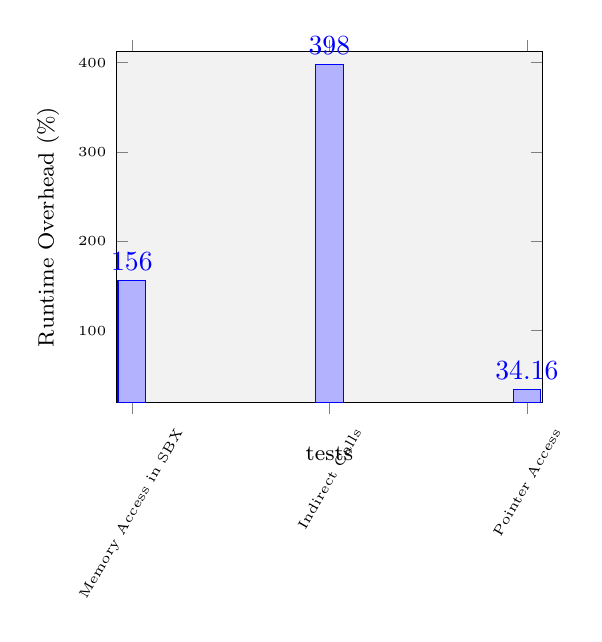
\begin{tikzpicture}  
  
\begin{axis}  
[  
    ybar,  
    enlargelimits=0.04,  
    ylabel={Runtime Overhead (\%)}, % the ylabel must precede a # symbol.  
    %xlabel={Micro-Benchmark Tests},  
    symbolic x coords={Memory Access in SBX, Indirect Calls, Pointer Access}, % these are the specification of coordinates on the x-axis.  
    xtick=data,  
    bar width=10pt,
    width=7cm,
    x tick label/.append style={font=\tiny, rotate=30},
    y tick label/.append style={font=\tiny},
    axis background/.style={fill=gray!10},
    x label style={at={(axis description cs:0.5,-0.1)},anchor=north, font=\footnotesize},
    xlabel={tests},
    ylabel style={font=\footnotesize},
     nodes near coords, % this command is used to mention the y-axis points on the top of the particular bar.  
    nodes near coords align={vertical},  
    ]  
\addplot coordinates {(Memory Access in SBX,156) (Indirect Calls, 398) (Pointer Access, 34.16)};  
  
\end{axis}  
\end{tikzpicture} 
\caption{\systemname Micro-Benchmarks.}
\label{fig:microbenchmarks}
\end{figure}

\begin{figure}
\pgfplotsset{every x tick label/.append style={font=\tiny, rotate=30}}
\pgfplotsset{every y tick label/.append style={font=\tiny}}
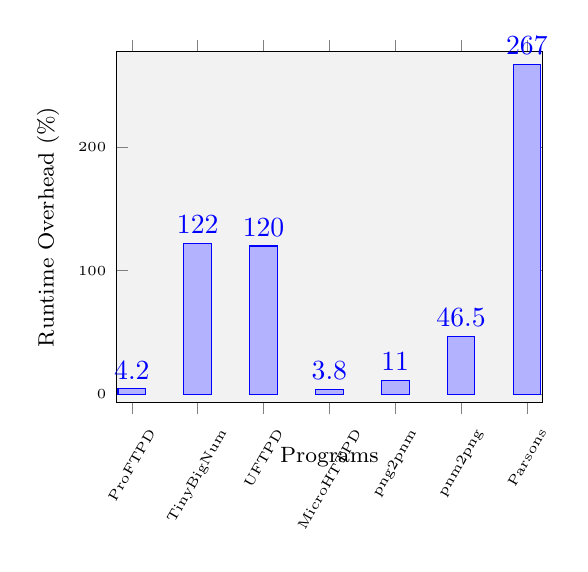
\begin{tikzpicture}  
  
\begin{axis}  
[  
    ybar,  
    enlargelimits=0.04,  
    ylabel={Runtime Overhead (\%)}, % the ylabel must precede a # symbol.  
    %xlabel={Programs},  
    symbolic x coords={ProFTPD, TinyBigNum, UFTPD, MicroHTTPD, png2pnm, pnm2png, Parsons}, % these are the specification of coordinates on the x-axis.  
    xtick=data,  
    bar width=10pt,
    width=7cm,
    x tick label/.append style={font=\tiny, rotate=30},
    y tick label/.append style={font=\tiny},
    axis background/.style={fill=gray!10},
    x label style={at={(axis description cs:0.5,-0.1)},anchor=north, font=\footnotesize},
    xlabel={Programs},
    ylabel style={font=\footnotesize},
     nodes near coords, % this command is used to mention the y-axis points on the top of the particular bar.  
    nodes near coords align={vertical},  
    ]  
\addplot coordinates {(ProFTPD,4.2) (TinyBigNum,122) (UFTPD, 120) (MicroHTTPD,3.8) (png2pnm, 11) (pnm2png, 46.5) (Parsons, 267)};  
  
\end{axis}  
\end{tikzpicture} 
\caption{Runtime Overhead of Partioned Programs.}
\label{fig:runtimeoverhead}
\end{figure}

